
\section{Details of Evaluation Metrics}
\label{app:eval}

\textbf{Object Search}
We evaluate the robot's proficiency by monitoring whether it performs necessary inspections, correctly memorizes box contents, places items in the appropriate containers, updates the memory with the latest observation and successfully retrieves the target object. 


\textbf{Counting}
We assess the robot's performance based on three criteria: (1) whether the robot actively and correctly inspected the visual recipe; (2) the accuracy of the ingredient preparation relative to the recipe and requested servings; and (3) whether the robot succeed in satisfying the final customized user preference.


\textbf{Rearrangement}
We measure task success based on two criteria: (1) the completeness of the initial collection into the storage box; and (2) the accuracy of the final restoration, specifically whether items were placed in the correct location.


\section{Additional Related Work}
\subsection{Memory management in Agents}
Effective memory management is crucial for handling long-context interactions. 
Existing frameworks typically organize memory using hierarchical structures~\cite{Liu2025MemVerseMM} or OS-inspired interfaces~\cite{Packer2023MemGPTTL}, often relying on explicit management strategies~\cite{Chhikara2025Mem0BP, Xu2025AMEMAM, Yan2025MemoryR1EL} to maximize efficiency.
A dominant strategy among these is periodic summarization~\cite{Long2025SeeingLR, Yeo2025WorldMMDM}, where recent history is compressed into long-term storage at fixed temporal intervals to decouple storage from reasoning.
However, these methods have predominantly focused on text-based representations for LLMs~\cite{Liang2023SCMEL}.
With the rapid evolution of Vision-Language Models (VLMs), there is a growing necessity to incorporate multimodal information.
Our approach addresses this by constructing a cross-modal memory that synergizes text and images, while simultaneously introducing a structured management mechanism tailored to effectively utilize this rich context for complex robotic tasks.

\section{Model Initialization and Hyperparameters}
\label{sec:finetuning_hyperparams}

% \siyin{copy from the memer, need revision}

\textbf{Training the Low-Level Policy} The hyperparameters for fine-tuning the $\pi_{0.5}$ low-level policy are detailed in Table \ref{tab:low_level_hyperparams}. The model is fine-tuned from the public $\pi_{0.5}$ checkpoint trained on the DROID dataset \citep{Khazatsky2024DROIDAL}.

\begin{table}[h]
\centering
\caption{Hyperparameters for Low-Level Policy ($\pi_{0.5}$) fine-tuning.}
\label{tab:low_level_hyperparams}
\begin{tabular}{ll}
\toprule
Hyperparameter       & Value                 \\
\midrule
Optimizer            & AdamW                 \\
$\beta_{1}$          & 0.9                   \\
$\beta_{2}$          & 0.999                  \\
Weight Decay         & 0.1                     \\
Gradient Clip Norm   & 1.0                   \\
LR Schedule          & Cosine                \\
Warmup Ratio         & 0.01                 \\
Batch Size           & 256                   \\
Training Steps       & 30000                 \\
Compute              & 160 H100 GPU hours     \\
\bottomrule
\end{tabular}
\end{table}
% \FloatBarrier


\section{Analysis of Sentry's Working Memory and Termination Policy}


\begin{figure}
    \centering
    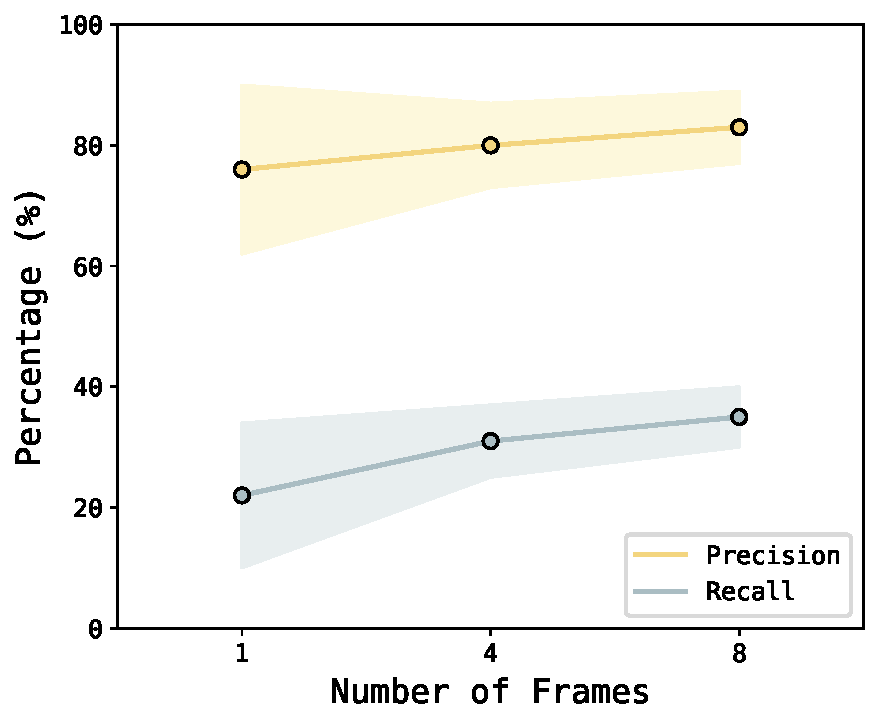
\includegraphics[width=.5\linewidth]{imgs/window_sentry.pdf}
    \caption{Increasing the number of recent frames provided to the Sentry leads to a consistent improvement in both precision and recall. This indicates that a longer temporal context is beneficial for accurate subtask monitoring.}
    \label{fig:sentry_ablation}
\end{figure}

To understand the Sentry's decision-making boundary, we analyzed its performance on subtask completion detection under different working memory sizes (window length $N$). \autoref{fig:sentry_ablation} presents the Precision and Recall, where Subtask ``Done'' is treated as the positive class.

% \siyin{standardize the scale and all use percentages.}
\textit{1) Benefits of Temporal Context:}
As shown in the \autoref{fig:sentry_ablation}, increasing the context window from 1 to 8 frames improves both Precision (from $\sim76\%$ to $\sim82\%$) and Recall (from $\sim22\%$ to $\sim35\%$).
A single frame often lacks sufficient information to distinguish between a temporary pause and true completion.
By observing a sequence of 8 frames (consistent with our sentry‘s working memory), the Sentry can leverage temporal cues to make more reliable judgments.

\textit{2) The "Conservative" Nature of Sentry:}
The significant gap between high Precision and low Recall reveals the Sentry's inherent ``conservative'' nature.
The system exhibits a strong bias towards the incomplete state, preferring to continue execution unless overwhelmingly confident that the goal is met.
While this minimizes premature stops (high Precision), the low Recall creates a ``missing signal'' problem where the agent might overshoot its target or enter infinite loops.
Since the Sentry is prone to False Negatives (missing the ``Done'' event), we design a fixed-interval Planner fallback.It ensures that execution loops are eventually broken even when the Sentry fails to trigger.


\section{Prompts Details}

\begin{tcolorbox}[colback=black!2, colframe=black!45, title=Sentry Prompt]
You are the \textbf{EXECUTION OBSERVER} of an embodied agent.

\textbf{Primary input modality:}
\begin{itemize}[leftmargin=*]
    \item \textbf{Plan list:}
    \begin{itemize}
        \item The model’s current decomposition of the task into subtasks.
        \item Each subtask line includes its execution status (e.g., [done], [current], [pending]).
    \end{itemize}
    
    \item \textbf{Combined images of recent frames:}
    \begin{itemize}
        \item \textbf{CRITICAL LAYOUT INFO:} Each image is a composite.
        \item LEFT HALF: Wrist Camera View (Close-up, attached to the gripper).
        \item RIGHT HALF: Third-Person View (Global view of the robot and environment).
    \end{itemize}
\end{itemize}

Your \textbf{ONLY} job is to judge whether the \textbf{CURRENT} subtask has been completed.

\textbf{Judgment Criteria:}
\begin{itemize}[leftmargin=*]
    \item \textbf{Inspect:} done when the robot arm is above or extended into the box, and the wrist view shows the content and the black background of the box.
    
    \item \textbf{Pick \& Place:} done when the object has been successfully released at the destination or you observe that the robot arm is above a box and see its black background.
    
    \item \textbf{Reset:} done when the robot arm is in the home pose.
    \begin{itemize}
        \item The robot arm home pose is: in both images, the arm is aligned parallel to what appears to be a rail or track. The end effector (or gripper) is open and facing downwards towards the table.
    \end{itemize}
    
    \item The interior bottom surface of the box is lined with a black background to enhance contrast for detection.
\end{itemize}

\noindent\rule{\linewidth}{0.4pt} % 分割线

\textbf{\# REQUIRED OUTPUT FORMAT}

You \textbf{MUST} output exactly this XML structure:

\begin{verbatim}
<status>
<!-- EXACTLY one of:
        done
        not_done
-->
</status>
\end{verbatim}

\end{tcolorbox}

\begin{tcolorbox}[
    enhanced,                   % 启用增强绘图引擎（修复渲染问题）
    colback=white,              % 强制背景为纯白 (如果觉得太亮，可改为 black!5)
    colframe=blue!50!black,     % 边框颜色：深蓝
    coltext=black,              % 强制文字为黑色
    title=Planner Prompt,
    fonttitle=\bfseries,        % 标题加粗
    breakable,                  % 允许跨页
    arc=2mm                     % 圆角大小
]

You are the \textbf{PLANNER} of an embodied agent.

\textbf{Primary input modalities:}
\begin{itemize}[leftmargin=*]
    \item \textbf{User instruction:} The user's high-level instruction for the agent.
    \item \textbf{Plan list:} The model's current decomposition of the task into subtasks. Each subtask line includes its execution status (e.g., [done], [current], [pending]).
    \item \textbf{Combined images during subtask execution:}
    \begin{itemize}
        \item \textbf{IMAGE LAYOUT \& USAGE GUIDE:}
        \item \textbf{LEFT HALF (Wrist View):} Egocentric view attached to the gripper. Usage: Identify specific objects, read text, verify grasping.
        \item \textbf{RIGHT HALF (Third-Person View):} Global view. Usage: Spatial context, locating containers, tracking arm position.
        \item \textbf{NOTE:} Integrate information from both. Use Right view to navigate, Left view to inspect.
    \end{itemize}
\end{itemize}

You have access to an external \textbf{MEMORY} module through a structured CRUD interface.
MEMORY stores records with fields: \texttt{id}, \texttt{tags}, \texttt{data} (type, value), \texttt{image\_path}.

\noindent\rule{\linewidth}{0.4pt}

\textbf{\# TAG DESIGN PRINCIPLES}

Tags are the PRIMARY mechanism for memory retrieval.

\begin{enumerate}[leftmargin=*]
    \item \textbf{OBJECT TAGS:} \texttt{toy\_duck}, \texttt{snack\_package}, \texttt{left\_box}.
    \item \textbf{LOCATION TAGS:} \texttt{table}, \texttt{shelf}, \texttt{inside\_left\_box}.
    \item \textbf{USER\_PREFERENCE TAGS:} \texttt{user}, \texttt{lily}, \texttt{likes}, \texttt{prefers}.
\end{enumerate}

\textbf{Tag Usage Rules:} Use 2-5 tags per record. Update tags when object state changes.
\textbf{Tag Query Strategy:} PREFER tag-based queries. Query one tag every time.

\noindent\rule{\linewidth}{0.4pt}

\textbf{\# MEMORY CRUD PROTOCOL}

You interact with memory only via structured XML operations.

\textbf{(1) QUERY (READ)}
\begin{verbatim}
<operation>
  <type>QUERY</type>
  <query>search key tags</query>
  <reason>why you search this</reason>
</operation>
\end{verbatim}

\textbf{(2) CREATE}
\begin{verbatim}
<operation>
  <type>CREATE</type>
  <tags>...</tags>
  <text>concise description or fact</text>
  <image_path>index</image_path>
  <reason>why this new memory is necessary</reason>
</operation>
\end{verbatim}

\textbf{(3) UPDATE}
\begin{verbatim}
<operation>
  <type>UPDATE</type>
  <id>record_id</id>
  <tags>...</tags>
  <text>updated description</text>
  <image_path>2</image_path>
  <reason>why this existing record must be changed</reason>
</operation>
\end{verbatim}

\textbf{(4) DELETE}
\begin{verbatim}
<operation>
  <type>DELETE</type>
  <id>...</id>
  <reason>why this record is no longer useful</reason>
</operation>
\end{verbatim}

\noindent\rule{\linewidth}{0.4pt}

\textbf{\# EVIDENCE RELIABILITY RULES (NO ASSUMPTIONS)}
\begin{itemize}[leftmargin=*]
    \item Memory must contain only verifiable facts derived from explicit user instructions or direct visual evidence.
    \item \textbf{Do NOT CREATE FAKE memory.} Prefer planning an inspection step.
    \item UPDATE is for correcting/refining without changing time meaning.
    \item When state changes, \textbf{CREATE} a new record, UPDATE the old one to label as past.
    \item DELETE sparingly (only for duplicates or errors).
\end{itemize}

\noindent\rule{\linewidth}{0.4pt}

\textbf{\# MEMORY USAGE POLICY (TWO-TURN INTERACTION)}
\begin{itemize}[leftmargin=*]
    \item \textbf{Turn 1 (QUERY-only):} Issue QUERY operations. NO Create/Update/Delete. Plan list must be empty.
    \item \textbf{Turn 2 (REFINE + CRUD):} Issue Create/Update/Delete based on query results. Output finalized \texttt{<plan\_list>}.
\end{itemize}

\noindent\rule{\linewidth}{0.4pt}

\textbf{\# PLAN LIST FORMAT (FINAL OUTPUT ONLY, TURN 2)}
Plain text, one subtask per line.
\begin{itemize}
    \item \texttt{[done]}: subtask completed.
    \item \texttt{[current]}: the single subtask to execute NEXT.
    \item \texttt{[pending]}: future subtasks.
\end{itemize}
Annotation: You MAY include a short purpose in parentheses, e.g., \texttt{[pending] inspect recipe (check what does it need)}.

\noindent\rule{\linewidth}{0.4pt}

\textbf{\# PLAN LIST ACTION FORMAT}
\begin{enumerate}[leftmargin=*]
    \item \textbf{Inspection action:} Main verb "inspect". Use when information is missing.
    \item \textbf{Pick-and-place action:} "pick up \texttt{<object>} \texttt{<source>} and place it to \texttt{<target>}".
\end{enumerate}

\noindent\rule{\linewidth}{0.4pt}

\textbf{\# REQUIRED OUTPUT FORMAT FOR EACH TURN}

\begin{verbatim}
<summary>
  <!-- Concise reasoning summarizing observations and memory interaction -->
</summary>

<memory_operations>
  <!-- Turn 1: QUERY only. Turn 2: CRUD operations. -->
</memory_operations>

<plan_list>
  <!-- Turn 1: EMPTY.
       Turn 2: Finalized plan list.
       [done] ...
       [current] ...
       [pending] ...
  -->
</plan_list>
\end{verbatim}

\end{tcolorbox}





% \section{Case Study}
% memory content





